\documentclass[../../../../main.tex]{subfiles}

\begin{document}

\section*{第1問}

\begin{proof}[解]
\begin{enumerate}
    \item[(1)] $p=0, t=2$ の時 $\min = 1$.

    \item[(2)] $f(t)=(p^2+1)t^2-4t+p^2+5$, $g(t)=t^2-2qt+q^2+\sqrt{3}$ とおく. $\{f(t)\}^2+\{g(t)\}^2=4$ だから,

    (1)から $1 \leqq f(t)$, 又 $g(t) \geqq (t-q)^2+\sqrt{3} \geqq \sqrt{3}$ だから,
    \[
    4 \leqq 1 + 3 = 4
    \]
    となり, 等号が成立. (1)から $p=0, t=2$ で, 又 $q=t=2$ である. よって
    \[
    (p, q) = (0, 2).
    \]
\end{enumerate}
\end{proof}

\section*{第2問}

\begin{proof}[解]
\begin{enumerate}
    \item[(1)] 準線のうち $x > 0$ のものを $l$ とする. $F(ae, 0)$ とおく時, この楕円の離心率は $e$ であり, 右図のように $P, H$ を定めると,
    \[
    \overline{PF} = e \overline{PH}
    \]
    だから, $\overline{PF} = r$ として,
    \[
    \frac{a}{e} - ae = r \cos \theta + \frac{r}{e}
    \]
    \[
    r = \frac{a(1-e^2)}{1+e\cos\theta}
    \]

    \begin{center}
    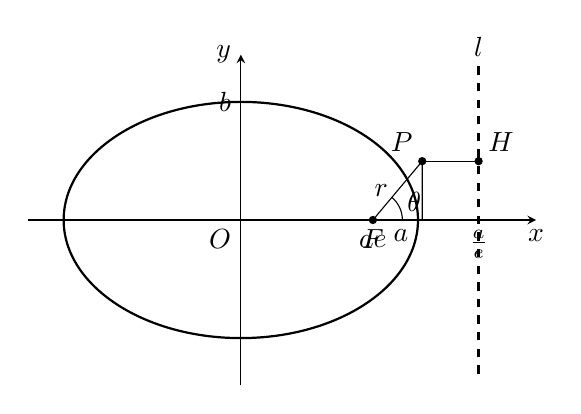
\begin{tikzpicture}[scale=1.5, >=stealth]
        % Axes
        \draw[->] (-1.8,0) -- (2.5,0) node[below] {$x$};
        \draw[->] (0,-1.4) -- (0,1.4) node[left] {$y$};
        \node[below left] at (0,0) {$O$};

        % Ellipse with a=1.5, b=1.0, e=0.745 => ae=1.118, a/e=2.013
        \draw[thick] (0,0) ellipse (1.5cm and 1.0cm);

        % Points and ticks
        \coordinate (F) at (1.118,0);
        \node[below] at (F) {$F$};
        \fill (F) circle (1pt);
        \node[below] at (1.118,-0.05) {$ae$};
        \node[below left] at (1.5,0) {$a$};
        \node[left] at (0,1.0) {$b$};

        % Directrix l
        \draw[dashed, thick] (2.013,-1.3) -- (2.013,1.3) node[above] {$l$};
        \node[below] at (2.013,0) {$\frac{a}{e}$};

        % Point P and H
        \coordinate (P) at ({1.118 + 0.65*cos(50)}, {0.65*sin(50)});
        \fill (P) circle (1pt);
        \node[above left] at (P) {$P$};

        \coordinate (H) at (2.013, {0.65*sin(50)});
        \fill (H) circle (1pt);
        \node[above right] at (H) {$H$};

        % Segments
        \draw (F) -- (P) node[midway, left] {$r$};
        \draw (P) -- (H);
        \draw (P) -- ({1.118 + 0.65*cos(50)}, 0);

        % Angle theta arc
        \draw (1.118+0.25,0) arc (0:50:0.25);
        \node at (1.118+0.35, 0.15) {$\theta$};
    \end{tikzpicture}
    \end{center}

    \item[(2)] $P, Q$ に対応する $\theta$ を $\alpha, \alpha+\pi \, (0 \leqq \alpha \leqq \pi)$, $R, S$ に対応する $\theta$ を $\alpha-\frac{\pi}{2}, \alpha+\frac{\pi}{2}$ とする. $A = a(1-e^2)$ とすると,
    \begin{align*}
        \overline{PF} \cdot \overline{QF} &= r(\alpha) \cdot r(\alpha+\pi) \\
        &= \frac{A}{1+e\cos\alpha} \cdot \frac{A}{1-e\cos\alpha} = \frac{A^2}{1-e^2\cos^2\alpha}
    \end{align*}
    \[
    \overline{FR} \cdot \overline{FS} = r\left(\alpha+\frac{\pi}{2}\right) r\left(\alpha-\frac{\pi}{2}\right) = \frac{A^2}{1-e^2\sin^2\alpha}
    \]
    だから
    \[
    \frac{1}{\overline{PF}\cdot\overline{QF}} + \frac{1}{\overline{FR}\cdot\overline{FS}} = \frac{2-e^2}{A^2} = \frac{2-e^2}{a^2(1-e^2)^2}.
    \]
\end{enumerate}
\end{proof}

\section*{第3問}

\begin{proof}[解]
$e(\theta) = \cos\theta + i \sin\theta$ とし, $S$ の $n$ 個の要素を $a_k = e(\theta_k) \; (k=1, 2, \dots, n)$ とする. さらに $a_1 = 1$ とする. (ii)で $(z, w) = (1, 1)$ として, $-1$ も $S$ の元である. そこで $a_2 = -1$ とする. よって $n \geqq 2$ である.

\begin{enumerate}
    \item[$1^\circ$] $n=2$

    $S = \{1, -1\}$ は (i), (ii) をみたす. よって十分である.

    \item[$2^\circ$] $n=3$

    $(z, w) = (a_3, 1)$ とおくと,
    \[
    p = a_3 - 2 \cos\theta_3 = -\cos\theta_3 + i \sin\theta_3
    \]
    が $S$ の元 $1, -1, a_3$ のいずれかに等しい.
    \[
    \begin{cases}
        p = 1 \iff \sin\theta_3 = 0 \land -\cos\theta_3 = 1 \iff a_3 = -1 \\
        p = -1 \iff a_3 = 1 \\
        p = a_3 \iff a_3 = \pm i
    \end{cases}
    \]
    だから, $a_3 \neq 1, -1$ とあわせて, $a_3 = \pm i$ が必要だが, $S = \{1, -1, i\}, \{1, -1, -i\}$ はいずれも (ii) をみたさず不適. ((ii)で $(z, w) = (i, i)$ or $(-i, -i)$ とすればわかる)

    \item[$3^\circ$] $n=4$

    $2^\circ$から, $a_3 = \pm i$ が必要である. まず, $a_3 = i$ とする. (ii)で $(z, w) = (i, i)$ として, $-i$ も $S$ の元である. さて, $S = \{\pm 1, \pm i\}$ は (i), (ii) をみたし十分で, $a_3 = -i$ の時も同じく, $(z, w) = (-i, -i)$ として $S = \{\pm 1, \pm i\}$ を得る.
\end{enumerate}

以上から $S = \{\pm 1\}, \{\pm 1, \pm i\}$.
\end{proof}

\section*{第4問}

\begin{proof}[解]
円の半径を $1$ とする. この円に内接する正 $k$ 角形の面積 $S_k$ は,
\[
S_k = k \cdot \sin \frac{\pi}{k} \cos \frac{\pi}{k} = \frac{k}{2} \sin \frac{2\pi}{k}.
\]
だから,
\begin{align*}
    &\frac{2}{3} S_{3n} < S_n < \frac{\sqrt{3}}{2} S_{2n} \\
    \iff &\frac{2}{3} \cdot \frac{3n}{2} \sin \frac{2\pi}{3n} < \frac{n}{2} \sin \frac{2\pi}{n} < \frac{\sqrt{3}}{2} \cdot \frac{2n}{2} \sin \frac{2\pi}{2n} \\
    \iff &\sin \frac{2\pi}{3n} < \frac{1}{2} \sin \frac{2\pi}{n} < \frac{\sqrt{3}}{2} \sin \frac{2\pi}{2n} \qquad \dots \text{\textcircled{1}}
\end{align*}

\begin{center}
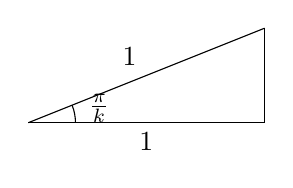
\begin{tikzpicture}[scale=1.5, >=stealth]
    \draw (0,0) -- (2,0) node[midway, below] {$1$};
    \draw (0,0) -- (2,0.8) node[midway, above left] {$1$};
    \draw (2,0) -- (2,0.8);
    \draw (0.4,0) arc (0:21.8:0.4);
    \node at (0.6, 0.12) {$\frac{\pi}{k}$};
\end{tikzpicture}
\end{center}

$t = \sin \frac{2\pi}{3n}$ とおく. \textcircled{1}の左側から
\[
t < \frac{1}{2}(3t - 4t^3)
\]
$t > 0$ から,
\[
2 < 3 - 4t^2 \quad \therefore 0 < t < \frac{1}{2} = \sin \frac{\pi}{6} \qquad \dots \text{\textcircled{2}}
\]
\textcircled{1}の右側から
\[
2 \sin \frac{\pi}{n} \cos \frac{\pi}{n} < \sqrt{3} \sin \frac{\pi}{n}
\]
$\sin \frac{\pi}{n} > 0$ から
\[
\cos \frac{\pi}{n} < \frac{\sqrt{3}}{2} \qquad \dots \text{\textcircled{3}}
\]
\textcircled{2}, \textcircled{3}を満たすのは,
\[
\frac{2\pi}{3n} < \frac{\pi}{6} \quad \land \quad \frac{\pi}{6} < \frac{\pi}{n}
\]
\[
\iff 4 < n < 6 \quad (\because n \in \mathbb{N})
\]
\[
\iff n = 5.
\]
\end{proof}

\section*{第5問}

\begin{proof}[解]
\begin{enumerate}
    \item[(1)] 帰納的に示す. $n=1$ の時は成立するので, 以下 $n=k \in \mathbb{N}$ での成立を仮定する.
    \[
    |\sin(k+1)\theta| \leqq |\sin k\theta||\cos\theta| + |\cos k\theta||\sin\theta| \leqq k\sin\theta + \sin\theta = (k+1)\sin\theta
    \]
    から $n=k+1$ でも成立. よって示された.

    \item[(2)] $0 \leqq f(\theta) \quad \dots \text{\textcircled{1}}$
    \[
    \int_0^\pi f(\theta) \sin\theta \, d\theta = 1 \quad \dots \text{\textcircled{2}}
    \]
    (1)及び\textcircled{1}から, $0 \leqq \theta \leqq \pi$ の時
    \[
    f(\theta) \sin n\theta \leqq f(\theta) |\sin n\theta| \leqq n f(\theta) \sin\theta
    \]
    だから, 同区間で積分して, \textcircled{2}から,
    \[
    \int_0^\pi f(\theta) \sin n\theta \, d\theta \leqq n.
    \]
\end{enumerate}
\end{proof}

\section*{第6問}

\begin{proof}[解]
\begin{enumerate}
    \item[(1)] $y = e^{mx}$ の時, $y' = my$ だから,
    \[
    3y' - 2y = 0 \iff (3m-2)y = 0 \iff m = \frac{2}{3} \quad (\because y \neq 0).
    \]

    \item[(2)] $y = e^{\frac{2}{3}x} \cdot u(x)$ と表す. $y' = e^{\frac{2}{3}x} \left(u'(x) + \frac{2}{3}u(x)\right)$ だから, ①に代入して
    \[
    3 e^{\frac{2}{3}x} \left(u'(x) + \frac{2}{3}u(x)\right) - 2 e^{\frac{2}{3}x} u(x) = e^x
    \]
    \[
    3 u'(x) = e^{\frac{1}{3}x}
    \]
    両辺積分して,
    \[
    u(x) = e^{\frac{1}{3}x} + C.
    \]

    \item[(3)] (2)で $y = e^x + C \cdot e^{\frac{2}{3}x}$ で, $x=0$ で $y=10$ となるようにして,
    \[
    10 = 1 + C \quad \therefore C = 9.
    \]
    だから,
    \[
    y = e^x + 9 e^{\frac{2}{3}x}.
    \]
\end{enumerate}
\end{proof}

\end{document}
